\section{Time Series Plot: Visualizing Trends Over Time}

Time series plots are essential tools in climate data analysis, allowing researchers to observe and interpret variations in a variable over time. A time series consists of data points collected or recorded at successive time intervals typically days, months, or years.

In climate science, variables such as temperature, precipitation, humidity, and pressure are often monitored over long periods. Plotting these values against time helps to identify seasonal patterns, trends, anomalies, and long-term climate changes.

Time series plots make it easier to detect cycles (like monsoon seasons), abrupt changes (such as droughts or floods), and overall trends (such as rising temperatures due to climate change). They are also useful for comparing trends across multiple locations or climate indicators.

In this section, we use R to generate time series plots using the \texttt{ggplot2} package. These plots provide a visual summary of climate variables, offering intuitive insights into their temporal behavior.

\subsection*{Precipitation and Temperature Over Time}

The following R code generates a time series plot comparing precipitation and temperature over time, using different colors for each variable.

\begin{verbatim}
ggplot(df_climate, aes(x = Date)) +
  geom_line(aes(y = Precip, color = 'Precipitation'), linewidth = 1) +
  geom_line(aes(y = Temp_2m, color = 'Temperature'), linewidth = 1) +
  labs(title = 'Precipitation and Temperature Over Time',
       x = 'Date',
       y = 'Values') +
  scale_color_manual(name = 'Legend', 
    values = c('Precipitation' = 'blue', 'Temperature' = 'orange')) +
  theme(legend.position = 'top')  # Adjust legend position as needed
\end{verbatim}

% Figure here---------------------------
\begin{figure}[h]
\centering
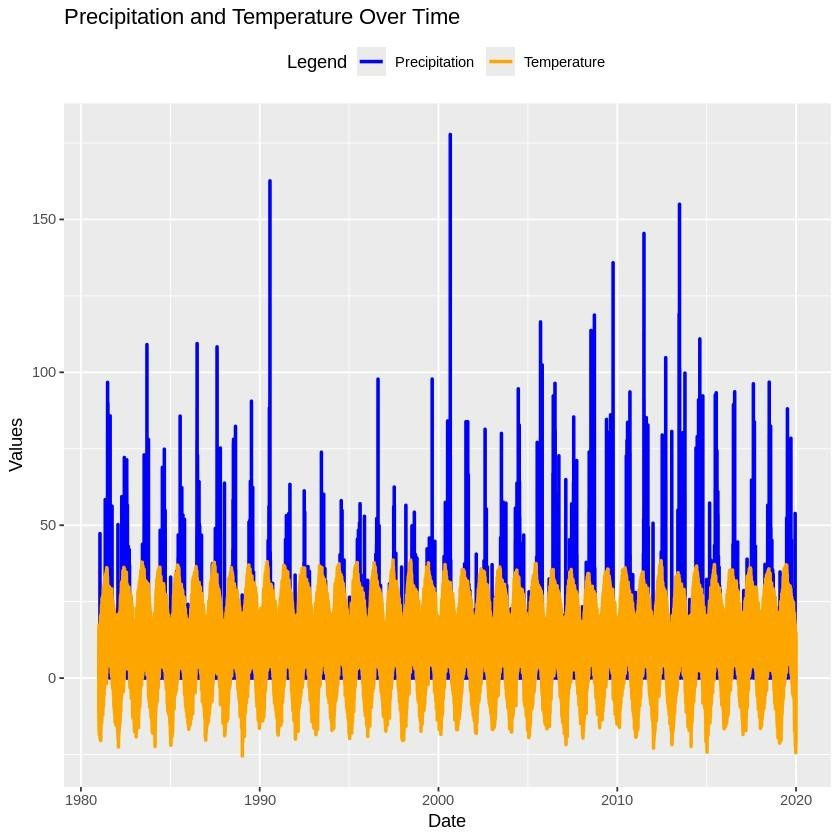
\includegraphics[width=0.5\textwidth]{figures/temp_precipt.jpg}
\caption{Temperature and Precipitation Over Time}
\end{figure}

\subsection*{Yearly Trend Analysis of Temperature}

The R code below calculates average temperature, precipitation, and humidity per year and plots the temperature trend over time with a smoothed line.

\begin{verbatim}
df_yearly <- df_climate %>%
  group_by(Year = format(Date, "%Y")) %>%
  summarise(
    AvgTemp = mean(Temp_2m, na.rm = TRUE),
    AvgPrecip = mean(Precip, na.rm = TRUE),
    AvgHumidity = mean(Humidity_2m, na.rm = TRUE)
  )

# Plot the trend over years
ggplot(df_yearly, aes(x = as.numeric(Year), y = AvgTemp)) +
geom_line(color = "blue", size = 1) + 
geom_point(color = "red") +  
geom_smooth(method = "loess", color = "darkgreen", 
linetype = "dashed", size = 1, se = FALSE) +# Smoothed trend line
labs(title = "Trend Analysis of Temperature Over Years",
       x = "Year",
       y = "Average Temperature (°C)") +
scale_x_continuous(
breaks = seq(min(df_yearly$Year),
max(df_yearly$Year), by = 2)) +  # Set interval
theme_minimal() +
theme(axis.text.x = element_text(angle = 45, hjust = 1))
\end{verbatim}

% Figure here-----------------------------
\begin{figure}[h]
\centering
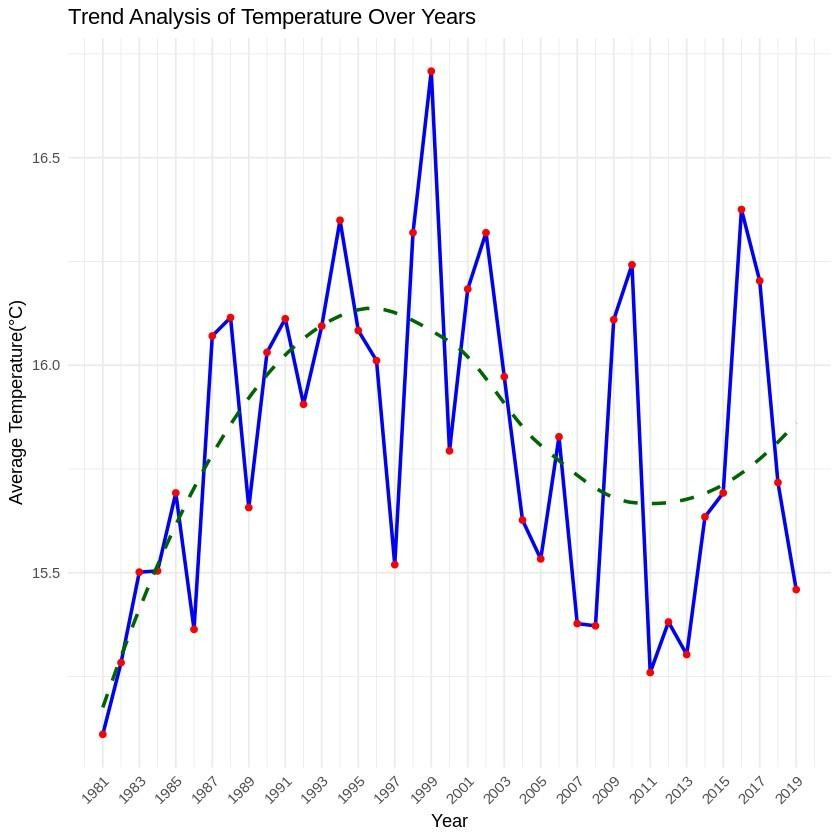
\includegraphics[width=0.5\textwidth]{figures/temp_trend.jpg}
\caption{Temperature Trend Over Years}
\end{figure}

\subsection*{Yearly Trend Analysis of Precipitation}

This R script shows how average precipitation changes over time using a line and smoothed trend plot.

\begin{verbatim}
# Plot the trend over years
ggplot(df_yearly, aes(x = as.numeric(Year),
y = AvgPrecip)) +
  geom_line(color = "blue", size = 1) +    
  geom_point(color = "red") +           
  geom_smooth(method = "loess", color = "darkgreen", 
              linetype = "dashed", size = 1, se = FALSE) +  
  labs(title = "Trend Analysis of Precipitation Over Years",
       x = "Year",
       y = "Average Precipitation (mm/day)") +
  scale_x_continuous(
  breaks = seq(min(df_yearly$Year),
  max(df_yearly$Year), 
  by = 2)) +  # Set interval
  theme_minimal() +
  theme(axis.text.x = element_text(angle = 45, hjust = 1))
\end{verbatim}

% figure here--------------------------
\begin{figure}[h]
\centering
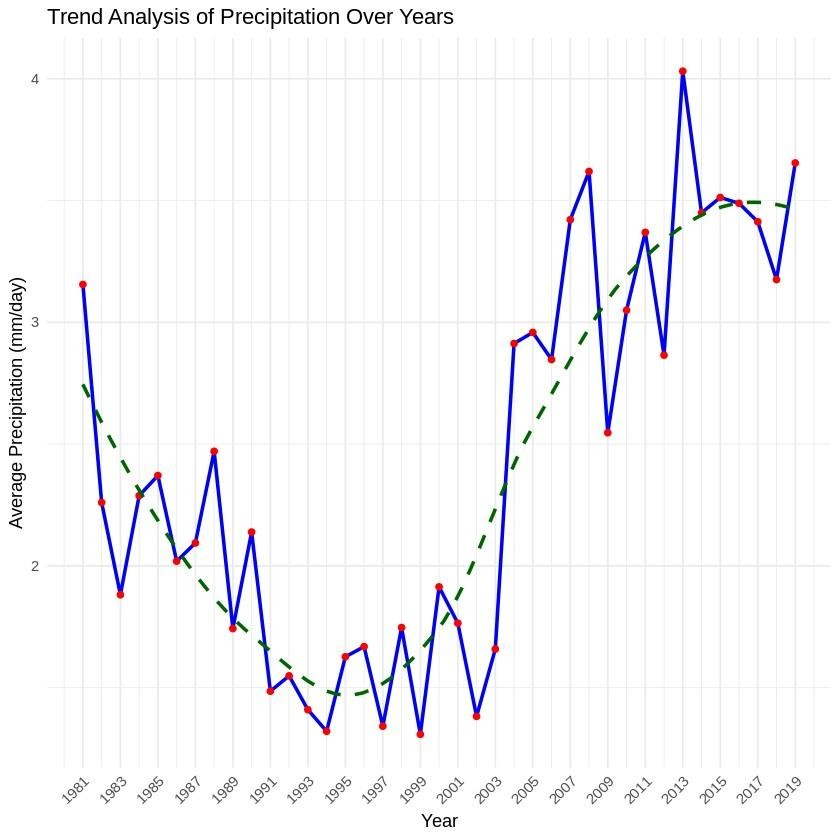
\includegraphics[width=0.5\textwidth]{figures/precip_trend.jpg}
\caption{Precipitation Trend Over Years}
\end{figure}
